%% Exemplo de utilizacao do estilo de formatacao normas-utf-tex (http://normas-utf-tex.sourceforge.net)
%% Autores: Hugo Vieira Neto (hvieir@utfpr.edu.br)
%%          Diogo Rosa Kuiaski (diogo.kuiaski@gmail.com)
%% Colaboradores:
%%          Cézar M. Vargas Benitez <cesarvargasb@gmail.com>
%%          Marcos Talau <talau@users.sourceforge.net>


%\documentclass[openright]{normas-utf-tex} %openright = o capitulo comeca sempre em paginas impares
\documentclass[oneside]{normas-utf-tex} %oneside = para dissertacoes com numero de paginas menor que 100 (apenas frente da folha) 

\usepackage[alf,abnt-emphasize=bf,bibjustif,recuo=0cm, abnt-etal-cite=2, abnt-etal-list=99]{abntcite} %configuracao correta das referencias bibliograficas.

\usepackage[brazil]{babel} % pacote portugues brasileiro
\usepackage[utf8]{inputenc} % pacote para acentuacao direta
\usepackage{amsmath,amsfonts,amssymb} % pacote matematico
\usepackage{graphicx} % pacote grafico
\usepackage{times} % fonte times

%Podem utilizar GEOMETRY{...} para realizar pequenos ajustes das margens. Onde, left=esquerda, right=direita, top=superior, bottom=inferior. P.ex.:
%\geometry{left=3.0cm,right=1.5cm,top=4cm,bottom=1cm} 

% ---------- Preambulo ----------
\instituicao{Universidade Tecnol\'ogica Federal do Paran\'a} % nome da instituicao
\programa{Departamento Acadêmico de Eletrônica} % nome do programa
\area{Inform\'atica Industrial} % [Engenharia Biom\'edica] ou [Inform\'atica Industrial] ou [Telem\'atica]

\documento{Monografia} % [Disserta\c{c}\~ao] ou [Tese]
\nivel{Mestrado} % [Mestrado] ou [Doutorado]
\titulacao{Mestre} % [Mestre] ou [Doutor]

\titulo{\MakeUppercase{Robô Explorador de Ambientes}} % titulo do trabalho em portugues
\title{\MakeUppercase{Ambience Explorer Robot}} % titulo do trabalho em ingles

\autor{Luis Guilherme Machado Camargo} % autor do trabalho
\autordois{Marcelo Teider Lopes}
\autortres{Matheus Silva Araújo}
\cita{CAMARGO, Luis Guilherme M. ; LOPES, Marcelo Teider; ARAÚJO, Matheus Silva} % sobrenome (maiusculas), nome do autor do trabalho

\palavraschave{Robótica, Exploração, Reconhecimento de Imagens, Sensores ...} % palavras-chave do trabalho
\keywords{Robotics, Exploration, Image Recognition, Sensors ...} % palavras-chave do trabalho em ingles

%\comentario{\UTFPRdocumentodata\ apresentada ao \UTFPRdocumentodata\ da \ABNTinstituicaodata\ como requisito parcial para obten\c{c}\~ao do grau de ``\UTFPRtitulacaodata\ em Ci\^encias'' -- \'Area de Concentra\c{c}\~ao: \UTFPRareadata.}

\comentario{\UTFPRdocumentodata\ apresentada ao Departamento Acadêmico de Eletrônica da \ABNTinstituicaodata\ como requisito parcial para aprovação na Disciplina de Oficina de Integração 2.}


\orientador[Orientadora:]{Profa. Dra. Myriam Regattieri De Biase da Silva Delgado} % nome do orientador do trabalho
%\orientador[Orientadora:]{Nome da Orientadora} % <- no caso de orientadora, usar esta sintaxe
%\coorientador{Nome do Co-orientador} % nome do co-orientador do trabalho, caso exista
%\coorientador[Co-orientadora:]{Nome da Co-orientadora} % <- no caso de co-orientadora, usar esta sintaxe
%\coorientador[Co-orientadores:]{Nome do Co-orientador} % no caso de 2 co-orientadores, usar esta sintaxe
%\coorientadorb{Nome do Co-orientador 2}	% este comando inclui o nome do 2o co-orientador

\local{Curitiba} % cidade
\data{\the\year} % ano automatico


%---------- Inicio do Documento ----------
\begin{document}

\capa % geracao automatica da capa
\folhaderosto % geracao automatica da folha de rosto
%\termodeaprovacao % <- ainda a ser implementado corretamente

% dedicatória (opcional)
%\begin{dedicatoria}
%Texto da dedicat\'oria.
%\end{dedicatoria}

% agradecimentos (opcional)
\begin{agradecimentos}
Este trabalhado não teria sido possível sem o projeto anteriormente apresentado por Bruno Meneguele, Fernando Padilha e Vinicius Arcanjo.
Por emprestar o robô e pelos diversos esclarecimentos (muitas vezes sobre assuntos que não os envolviam) nosso muito obrigado.

À Professora Myriam nosso agradecimento por aceitar o desafio de nos orientar e a atenção dispensada. 

Aos Professores Hugo Vieira e Mário Sérgio pela oportunidade sem par de aprendizado.

Aos Professores João Fabro e Celso Kaestner por permitirem o uso das dependências e recursos do Laboratório de Arquitetura de Computadores para a realização do projeto.

Aos colegas Lucas Campiolo Paiva e Cláudio Akio pela colaboração ocasional com o projeto.

Aos marceneiros do Almoxarifado da UTFPR pela ajuda com a construção do suporte da câmera.
 
\end{agradecimentos}

% epigrafe (opcional)
\begin{epigrafe}
\begin{itemize}
	\item \textbf{1ª lei:} Um robô não pode ferir um ser humano ou, por inacção, permitir que um ser humano sofra algum mal.
	\item \textbf{2ª lei:} Um robô deve obedecer às ordens que lhe sejam dadas por seres humanos, exceto nos casos em que tais ordens contrariem a Primeira Lei.
	\item \textbf{3ª lei:} Um robô deve proteger sua própria existência, desde que tal proteção não entre em conflito com a Primeira e Segunda Leis.
	\newline
	\item \textbf{Lei Zero:} Um robô não pode fazer mal à humanidade e nem, por inacção, permitir que ela sofra algum mal.
	\newline
	\newline
	\textit{Isaac Asimov}
\end{itemize}

\end{epigrafe}

%resumo
\begin{resumo}
Neste projeto foi realizada uma tentativa de desenvolver um robô explorador ambientes capaz de encontrar um objeto pré-definido em um ambiente controlado, ou explorar todo o ambiente caso não seja capaz de encontrá-lo. Posteriormente, o escopo do projeto foi alterado para um robô capaz de localizar um objeto em seu campo de visão e seguí-lo, como passo inicial para a construção de um robô explorador. Para tal usamos como sensor principal uma câmera, a \textit{CMUCam3}, desenvolvida pela \textit{Carmegie Mellon University}. Uma bússola também foi estudada como sensor auxiliar, para obter a direção do robô. A versão inicial do robô foi desenvolvido em \cite{Robo2d}.
\end{resumo}

%abstract
\begin{abstract}
An attempt to develop an explorer robot is made in this project, which would be capable of both finding a predefined object on a small, controlled, environment, and exploring the whole environment if it can't find it. Later the scope of the project was changed to a robot capable of finding an object at his line of vision and following it, as a inicial step in order to build an explorer robot.  A camera was used as the main sensor, the \textit{CMUCam3}, developed by \textit{Carmegie Mellon University}. A compass would also be used as an auxiliary sensor, in order to obtain the direction of the robot. The initial version of the Robot is developed in \cite{Robo2d}.
\end{abstract}

% listas (opcionais, mas recomenda-se a partir de 5 elementos)
\listadefiguras % geracao automatica da lista de figuras
\listadetabelas % geracao automatica da lista de tabelas
%\listadesiglas % geracao automatica da lista de siglas
%\listadesimbolos % geracao automatica da lista de simbolos

% sumario
\sumario % geracao automatica do sumario


%---------- Inicio do Texto ----------
% recomenda-se a escrita de cada capitulo em um arquivo texto separado (exemplo: intro.tex, fund.tex, exper.tex, concl.tex, etc.) e a posterior inclusao dos mesmos no mestre do documento utilizando o comando \input{}, da seguinte forma:
%\input{intro.tex}
%\input{fund.tex}
%\input{exper.tex}
%\input{concl.tex}


% ========== %
% INTRODUÇÃO %
% ========== %

\chapter{Introdução}

Robôs autônomos são aqueles capazes de realizar um objetivo desejado em um determinado ambiente sem a intervenção humana.

Robôs exploradores têm como objetivo explorar um ambiente até atingir uma finalidade específica sem se perder ou colidir com obstáculos.

Para isso, esses robôs utilizam sensores para percepção do ambiente e algoritmos inteligentes para tomada de decisões.

\section{Motivação}

Robôs autônomos exploradores têm diversas áreas de aplicação, desde atividades em hospitais a explorações planetárias. 

A possibilidade de aplicar diversas áreas de conhecimento do curso, de eletrônica a inteligência artificial, motivaram a equipe a escolher esse projeto. O subsídio de um robô já desenvolvido e a possibilidade de utilizar um sensor inteligente (\textit{CMUcam3}) viabilizaram o projeto.

\section{Objetivo}

O objetivo do projeto é a construção de um robô explorador, utilizando uma câmera e uma bússola como sensores. Ele deve ser capaz de identificar um objeto especifico e posteriormente explorar o ambiente onde se encontra a procura do objeto, caso este saia de seu campo de visão.

\subsection{Objetivo Geral}

Para o projeto atual, o ambiente de exploração será limitado a um retângulo de 168,2 cm por 118,9 cm, dimensões somadas de duas folhas tamanho A0, que serão utilizadass lado a lado para composição da arena de exploração. A cor branca das folhas irá determinar o chão para o robô. Eventualmente, podem ser colocados referenciais de fácil identificação (círculos de determinadas cores, por exemplo) nas extremidades da arena para melhor auto-localização do robô.


\subsection{Objetivos Específicos}

Entre os diversos objetivos específicos e objetos de estudo do projeto estão:

\begin{itemize}

    \item {Trabalhar com robótica;}

    \item {Trabalhar com sensores diversos;}

    \item {Comunicar diferentes dispositivos eletrônicos;}

    \item {Trabalhar com inteligência artificial;}

    \item {E por fim, unir esses conhecimentos para construção do robô.}


\end{itemize}


% ================ %
% DESCRIÇÃO DO ROBÔ %
% ================ %

\chapter{Sistema Mecânico}

O robô utilizado no projeto é o mesmo robô construído durante o projeto \textbf{Robô Explorador de Labirintos 2D} \cite{Robo2d} desta mesma disciplina.

No projeto original o robô era utilizado para explorar e solucionar labirintos em duas dimensões feitos através de trilhas pretas em um chão branco, utilizado emissores e sensores de luz infravermelha para identificar a pista. 

Todo o projeto mecânico foi reutilizado neste trabalho, incluindo rodas, caixa de redução e chassi. Foram reutilizados também o sistema de alimentação e a uma placa \textit{Arduíno Duemilanove}; o conjunto de sensores do robô original foi substituído por uma câmera \textit{CMUCam3}.

\section{Projeto Mecânico}

O diagrama do projeto físico do robô é apresentado na Figura \ref{int_fig01}.

\begin{figure}[h!]
    \center
    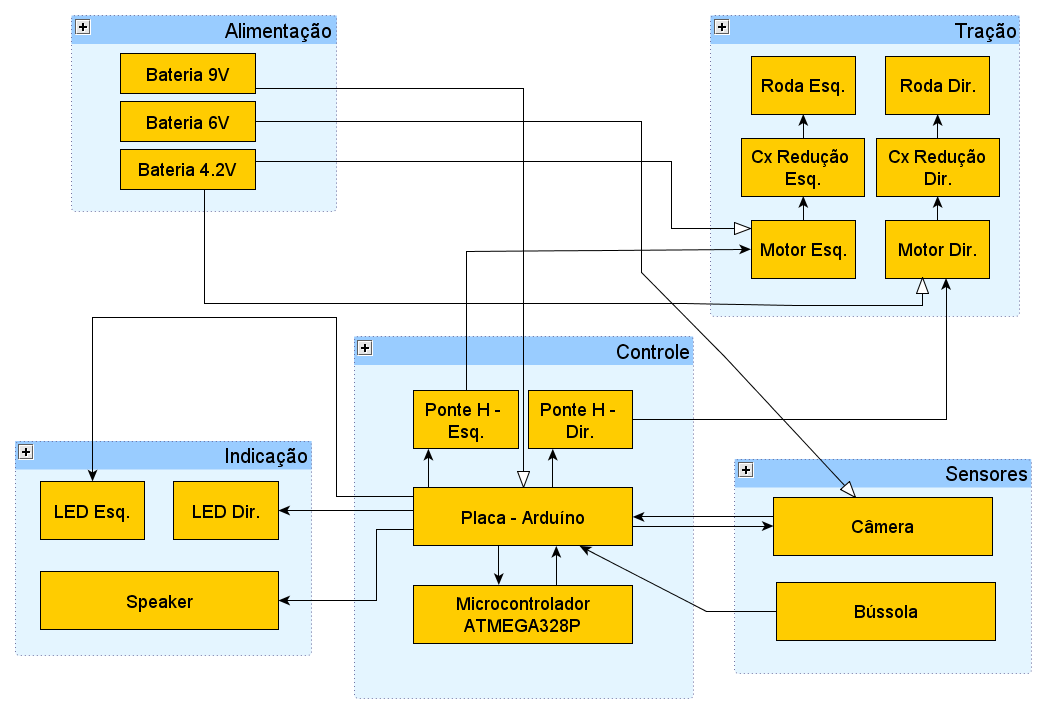
\includegraphics[scale=0.35]{imagens/robo_geral.png}
    \caption{Diagrama do Robô}
    \label{int_fig01}
\end{figure}

\subsection{Sistema de Alimentação}

Conjunto de baterias utilizadas como alimentação do robô.

\subsubsection{Bateria de 9V}
Utilizada para alimentação do \textit{Arduíno Duemilanove}, uma bateria PP3.

\subsubsection{Bateria de 4,2V}
Usada na alimentação dos motores, bateria de câmera fotográfica digital.

\subsubsection{Bateria de 6V}
Usada na alimentação da CMUCam3, quatro pilhas AA em série.

\subsection{Sistema de Indicação}

LEDs e \textit{Speaker} usados para indicar as ações do robô.

\subsubsection{LEDs}
Usados para indicação dos estados do robô, detalhados na Tabela \ref{int_tbl01}

\subsubsection{Speaker}
Utilizado como indicador sonoro de estados específicos do sistema, como reconhecimento do objeto e início e fim da busca do mesmo.

\subsection{Sistema de Tração}

Para tração do robô foi construído um sistema baseado em um motor elétrico e duas rodas centrais.

\subsubsection{Motores}
Motor elétrico de corrente contínua \textit{Mabuchi FA-130RA} de 3V com rotação de 12300 rpm, ou 205 voltas por segundo \cite{Robo2d}

\subsubsection{Caixas de redução}
Acopladas ao motor e às rodas reduzem a rotação do motor para que seja possível acionar as rodas. Na configuração usada, a redução é de 344:1 \cite{Robo2d}.

\subsubsection{Rodas}
O robô utiliza duas rodas \textit{off-road} em seu centro e uma esfera com giro livre atrás para manter o equilíbrio.

Com a rotação de 205 voltas/segundo e a redução de 344:1, a roda completa 0,6 voltas por segundo.

\subsection{Sistema de Controle}

Sistema para controle da movimentação do robô.

\subsubsection{Ponte H} 

A Ponte H é um circuito que permite a um microcontrolador acionar um motor de corrente contínua. Por questões eletrônicas \cite{Robo2d}, o circuito utilizado no projeto foi construído a partir de componentes discretos.

\subsubsection{Arduíno Duemilanove}

Placa \textit{Arduíno} utilizada no projeto anterior e reutilizada no projeto atual. Faz o interfaceamento dos diversos sistemas do projeto, \textit{i.e.}, recebe as decisões tomadas pelo Sistema de Navegação, embarcado na câmera, e aciona os motores para que o robô as execute. Seu funcionamento é detalhado na seção \ref{sec_arduino}.

\subsubsection{Microcontrolador ATMEGA328P}

Microcontolador presente da \textit{Arduíno Duemilanove}, os códigos construídos para controle do robô (Seção \ref{sec_soft_controle}) serão executados por ele.

\subsection{Sensores}

São apresentados na seção \ref{sec_sensores}.

\subsubsection{Câmera}

Ver seção \ref{sec_camera}.

\subsubsection{Bússola}

Ver seção \ref{sec_bussola}.

\section{Plataforma Arduíno}
\label{sec_arduino}

Arduíno é uma plataforma \textit{open-source} para prototipagem eletrônica que busca facilitar a construção de sistemas onde haja interação com objetos e o ambiente. \cite{arduino1}

Para o projeto \textbf{Robô Explorador de Labirintos 2D} foi utilizado uma placa \textit{Arduíno Duemilanove} que foi reutilizada no trabalho atual.

Dentro do projeto, o \textit{Arduíno} exerce um papel central de receber, via comunicação serial, as decisões tomadas pelo Sistema de Exploração, embarcado na câmera, e atuar sobre os motores através da Ponte H. Além disso, ele recebe o sinal lido através da bússola e aciona os dispositivos de indicação. Esse processo é representado na Figura \ref{int_fig02}.

\begin{figure}[h!]
    \center
    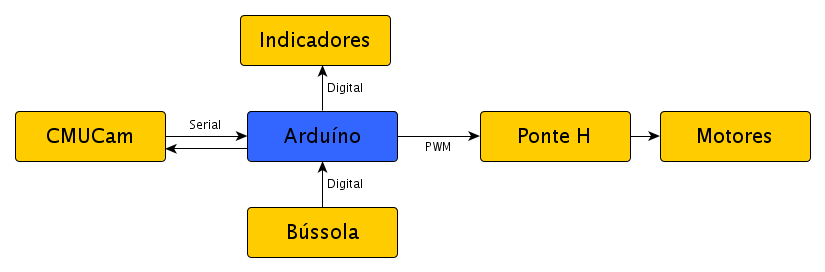
\includegraphics[scale=0.5]{imagens/processo_arduino.png}
    \caption{Processo de Comunicação - Arduíno}
    \label{int_fig02}
\end{figure}

O \textit{Arduíno Duemilanove} possui um microprocessador \textit{ATMEGA328P}, sua programação pode ser feita utilizando a linguagem de programação própria, baseada em \textit{Wiring} \cite{arduino1}. No entanto, é possível utilizar \textit{C++} para construir bibliotecas próprias utilizando também as bibliotecas já prontas do \textit{Arduíno}, e essa foi a opção feita pela equipe. O software de controle é detalhado na Seção \ref{sec_soft_controle}.

Para o interfaceamento com os diversos módulos do sistema, o \textit{Arduíno Duemilanove} possui 14 pinos de comunicação digital \cite{arduino2}, a configuração e utilização desses pinos está resumida na Tabela \ref{int_tbl02}.

\begin{table}[h!]
    \centering
    \begin{tabular}{|c|c|c|c|} \hline
        \textbf{Pino} & \textbf{Sentido do Sinal} & \textbf{Tipo de Comunicação} & \textbf{Função} \\ \hline
        00 & (RX) & Serial & Comunicação Câmera \\ \hline
        01 & (TX) & Serial & Comunicaçao Câmera \\ \hline
        02 & Entrada & Digital TTL & Bússola - Pino 1 \\ \hline
        03 & Entrada & Digital TTL & Bússola - Pino 4 \\ \hline
        04 & Saída & Digital TTL &LED Direito \\ \hline
        05 & Saída & Sinal PWM & Motor Esquerdo - Pino 2 \\ \hline
        06 & Saída & Sinal PWM & Motor Esquerdo - Pino 1 \\ \hline
        07 & Entrada & Digital TTL & Bússola - Pino 3 \\ \hline
        08 & Entrada & Digital TTL & Bússola - Pino 2 \\ \hline
        09 & Saída & Digital TTL & \textit{Speaker} \\ \hline
        10 & Saída & Sinal PWM & Motor Direito - Pino 2 \\ \hline
        11 & Saída & Sinal PWM & Motor Direito - Pino 1 \\ \hline
        12 & Saída & Digital TTL & LED Esquerdo \\ \hline
        13 & - & - & \textit{Não utilizado} \\ \hline
    \end{tabular}
    \caption{Pinos da placa \textit{Arduíno Duemilanove}}
    \label{int_tbl02}
\end{table}

\subsection{Comunicação com Indicadores}

Os indicadores do robô são os LEDs, esquerdo e direito, e o \textit{Speaker}. 

Os estados possíveis dos LEDs são aceso ou apagado, como visto na Tabela \ref{int_tbl01}. Para produzir os dois estados, é utilizada uma comunicação digital TTL, em que um sinal baixo (\textit{LOW}) produzirá o estado apagado e o sinal alto (\textit{HIGH}) irá deixar o LED aceso.

\begin{table}[h!]
    \centering
    \begin{tabular}{|c|c|c|} \hline
        \textbf{Estado} & \textbf{LED Esquerdo} & \textbf{LED Direito} \\ \hline
        Parado & Apagado & Apagado \\ \hline
        Andando para frente & Aceso & Aceso \\ \hline
        Virando para esquerda & Aceso & Apagado \\ \hline
        Virando para direita & Apagado & Aceso \\ \hline
    \end{tabular}
    \caption{Sistema de Indicação}
    \label{int_tbl01}
\end{table}

O LED Direito é ligado no pino 04 e o Esquerdo no 12.

Para o \textit{Speaker} é gerado um sinal com \textit{duty-cycle} de 50\% numa frequência especificada através da função \textit{tone} presente na biblioteca básica do \textit{Arduíno}.

O Speaker é ligado ao \textit{Arduíno} através do pino 09.

\subsection{Comunicação com Bússola}

A bússola utilizada pela equipe é a \textit{Dinsmore Sensor Modelo \#1490}, uma bússola digital com precisão de 45 graus, ou oito estados \cite{bussola}.

A \textit{Dinsmore \#1490} gera quatro sinais digitais TTL, a combinação desses sinais fornece a orientação lida pela bússola.

Os quatro sinais são ligados nos pinos 02, 03, 07 e 08 do \textit{Arduíno}.

Para funcionamento detalhado da bússola, ver seção \ref{sec_bussola}.

\subsection{Acionamento dos Motores}
\label{sec_com_motores}

Para acionamento dos motores, são utilizadas Pontes H, circuitos eletrônicos que permitem o acionamento por parte de um microcontrolador de um motor de corrente contínua em qualquer sentido de rotação. Por não ser objeto de estudo deste trabalho, seu funcionamento e a construção do circuito utilizado no robô não será explicitado, maiores informações podem ser encontradas em \cite{Robo2d} e \cite{ponteh}. 

A Ponte H, por sua vez, é acionada através de um sinal PWM - \textit{Pulse Width Modulation}. A modulação por largura de pulso é uma técnica usada para obter resultados analógicos com um sinal digital \cite{arduino3}. Uma onda quadrada é gerada, mudando o período em que essa onda está em ALTO (\textit{duty cycle}) é possível obter níveis médios de tensão diferentes. Assim, por exemplo, uma onda sempre em BAIXO, produrizá 0 V de nível médio de tensão, uma onda sempre em ALTO, 5 V; e uma onda 50\% do tempo em ALTO, 2,5 V. Esses diferentes níveis de tensão produzirão diferentes velocidades nos motores.

O \textit{Arduíno} possui portas que implementam o PWM, para utilizá-las é necessário usar a função \textit{analogWrite} que recebe como parâmetro um inteiro entre 0 e 255. Esse valor irá definir o tempo em que o sinal gerado ficará em ALTO.

Neste projeto, na maior parte dos movimentos, a velocidade do robô é constante, então foi definido experimentalmente o valor 127 para parâmetro da função \textit{analogWrite}, que produzirá um \textit{duty-cycle} de 50\%, e metade da velocidade do robô. Nos movimentos de correção do alinhamento do robô, esse valor é alterado para 40 ou 60\%.

Para cada Ponte H são gerados dois sinais que irão acionar os motores para frente ou para trás. Quando o sinal 1 é ALTO e o 2 é BAIXO, o motor gira num sentido, para frente, por exemplo; sinal 1 em BAIXO e sinal 2 em ALTO, ele gira no sentido inverto, para trás; esses sinais em função da ação executada pela robô são apresentados na tabela \ref{int_tbl03}.

\begin{table}[h!]
    \centering
    \begin{tabular}{|c|c|c|} \hline
        \textbf{Ação} & \textbf{Motor Esquerdo} & \textbf{Motor Direito} \\ \hline
        Parado & Desligado & Desligado \\ \hline
        Para frente & Frente & Frente \\ \hline
        Para trás & Trás & Trás \\ \hline
        Virando esquerda & Frente & Desligado \\ \hline
        Virando direita & Desligado & Frente \\ \hline
        Rotacionando esquerda & Frente & Trás \\ \hline
        Rotacionando direita & Trás & Frente \\ \hline
    \end{tabular}
    \caption{Acionamento dos Motores}
    \label{int_tbl03}
\end{table}

\subsection{Comunicação com CMUCam}

As decisões de movimentação são tomadas na aplicação que roda no microprocessador da câmera, no entanto quem aciona os motores e de fato produz o movimento é a aplicação executada no \textit{Arduíno}, por isso a necessidade de comunicação entre os dois dispositivos.

Esse interfaceamento entre o \textit{Arduíno} e a \textit{CMUCam} é feito através de comunicação serial assíncrona \textit{full-duplex}.

Por comunicação serial, entende-se aquela em que os \textit{bits} são enviados em \textit{fila} por um mesmo canal de comunicação. Por ser assíncrona, não há necessidade sincronismo de tempo entre os dois dispositivos envolvidos na comunicação, a própria mensagem irá definir o sinal de sincronismo. Como há necessidade de envio de mensagens da câmera para o \textit{Arduíno} e do \textit{Arduíno} para a câmera, a comunicação precisa ser \textit{full-duplex}, isso é, trafegar nos dois sentidos.

Para cada troca de mensagem será enviado um byte entre os dispositivos.

As mensagens que trafegarão da \textit{CMUCam} para o \textit{Arduíno} conterão comandos de ação para o robô, andar para frente ou para trás, rotacionar para a esquerda ou para a direita, parar o robô ou ainda corrigir o movimento do robô para determinado lado \footnote{Quando o movimento do robõ for por demais irregular e ele não conseguir seguir uma linha reta.}. E a câmera pode ainda requisitar ao \textit{Arduíno} a leitura de informação da bússola, nesse momento o \textit{Arduíno} envia para ela a informação do sensor.

Foram definidas constantes que serão enviadas de um dispositivo para o outro, apresentadas na Tabela \ref{int_tbl04}.

\begin{table}[htb!]
    \centering
    \begin{tabular}{|c|c|l|} \hline
        \textbf{Valor} & \textbf{Constante} & \textbf{Signficado} \\ \hline

        \multicolumn{3}{|c|}{\textit{Operações para o robô - Camêra-Arduíno}} \\ \hline
        1 & FORWARD & Movimenta robô para frente \\ \hline
        2 & BACKWARD & Movimenta robô para trás \\ \hline
        3 & SPINLEFT & Rotaciona robô para esquerda \\ \hline
        4 & SPINRIGHT & Rotaciona robô para direita \\ \hline
        5 & STOP & Pára robô \\ \hline
        6 & COMPASS & Executa leitura da bússola\\ \hline
        7 & ADJUSTLEFT & Corrige movimento do robô para esquerda \\ \hline
        8 & ADJUSTRIGHT & Corrige movimento do robô para direita \\ \hline
            
        \multicolumn{3}{|c|}{\textit{Leituras da bússola - Arduíno-Câmera}} \\ \hline
        1 & NORTH & Norte \\ \hline
        2 & NORTHEAST & Nordeste \\ \hline
        3 & EAST & Leste \\ \hline
        4 & SOUTHEAST & Sudeste \\ \hline
        5 & SOUTH & Sul \\ \hline
        6 & SOUTHWEST & Sudoeste \\ \hline
        7 & WEST & Oeste \\ \hline
        8 & NORTHWEST & Noroeste \\ \hline
    \end{tabular}
    \caption{Comunicação Arduíno-Câmera}
    \label{int_tbl04}

\end{table}


\section{Software de Controle}
\label{sec_soft_controle}

O Sistema de Controle executado no \textit{Arduíno} é responsável por receber e interpretar os comandos enviados pela \textit{CMUCam3} e atuar sobre os motores do robô produzindo o movimento necessário. Para executar essa tarefa, a equipe desenvolveu uma biblioteca orientada a objetos em \textit{C++}, cujo diagrama básico é apresentado na figura \ref{int_fig03}.

A ideia de construir a classe se baseia em representar em código a maneira como a equipe enxerga a função do \textit{Arduíno} e tentar encapsular as funções em classes que devem então ser apenas instanciadas, facilitando a programação, já que operações por vezes complexas são convertidas em operações elementares.

\begin{figure}[htb!]
    \center
    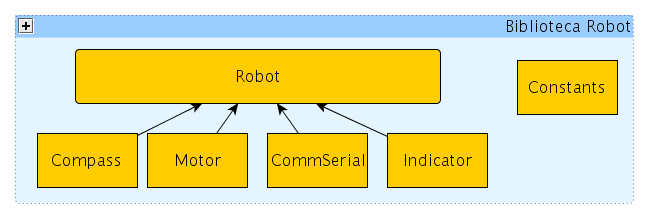
\includegraphics[scale=0.5]{imagens/diagrama_classe_robot.png}
    \caption{Diagrama - Biblioteca \textit{Robot}}
    \label{int_fig03}
\end{figure}

\subsection{Compass}

Classe responsável por fazer a leitura da bússola e decodificar o sinal lido, tendo como resposta apenas a constante que representa a direção cardeal lida.

\subsection{Motor}

Classe responsável por acionar os motores, recebe como parâmetro qual movimento deve ser feito e atua sobre os motores produzindo-o.

\subsection{CommSerial}

Classe para a comunicação com a \textit{CMUCam3}, possui um método de escrita e um de leitura apenas.

\subsection{Indicator}

Classe para produzir a representação necessária nos indicadores do robô.

\subsection{Robot}

Uma vez que todas as ações do robô estão definidas nas classes anteriormente citadas, a classe \textit{Robot} possui objetos das mesmas e sua tarefa é chamar as funções nos momentos adequados. 

No programa principal do \textit{Arduíno} há um objeto dessa classe que possui um método principal que funciona como um \textit{watchdog} para os comandos da \textit{CMUCam} através da classe \textit{CommSerial}, quando ele recebe um comando, dispara as funções das classes imediatamente abaixo.

\subsection{Constants}

Armazena as constantes definidas ao longo da biblioteca e não possui nenhum método. Armazena tanto as constantes de comunicação, Tabela \ref{int_tbl04}, quanto as constantes para acionamento dos motores, por exemplo.




% ======== %
% SENSORES %
% ======== %

\chapter{Sensores}
\label{sec_sensores}

A equipe utiliza dois sensores no projeto: um eletromagnético digital, Bússola; e um ótico, Câmera. O primeiro fornece informação de orientação do robô e o segundo informações visuais do ambiente.

\section{Bússola}
\label{sec_bussola}

A bússola utilizada no projeto é a \textit{Dinsmore Sensor Modelo \# 1490} \cite{bussola}, emprestada à equipe pelo professor Hugo Vieira.

Foi necessário construir um \textit{shield} para conectá-la ao \textit{Arduíno}. O circuito utilizado é apresentado na figura \ref{sen_fig01} e foi baseado no trabalho do \textit{Autonomous Vehicle Team} do \textit{College of New Jersey} \cite{newjersey}.

Internamente a bússola funciona como um transistor coletor aberto NPN e fornece sinais 0 ou 5V, TTL, \cite{bussola}, captados nos catodos dos diodos, para as entradas digitais do \textit{Arduíno}, sendo alimentada com 5V através do \textit{Arduíno} também.

\begin{figure}[h!]
    \center
    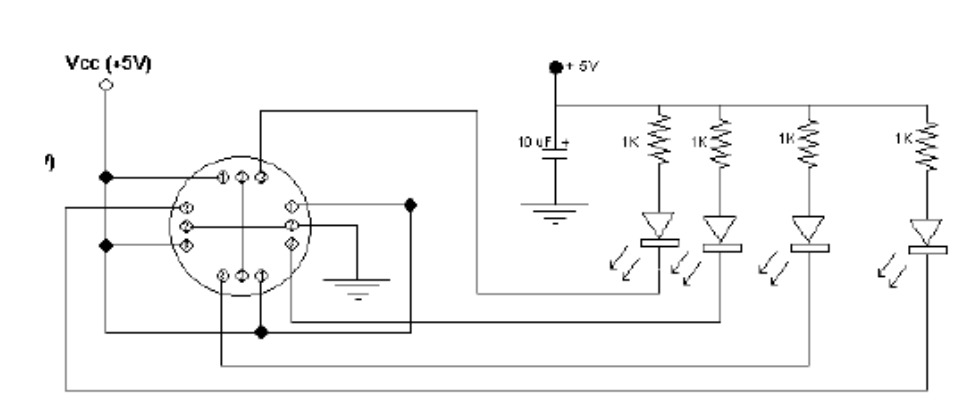
\includegraphics[scale=0.4]{imagens/circuito_bussola.png}
    \caption{Circuito Eletrônico - Bússola}
    \label{sen_fig01}
\end{figure}

A combinação dos quatro sinais fornecidos pela bússola fornece sua orientação com uma precisão de 45 graus, \textit{i.e.}, há oito estados possíveis para a bússola. 

A combinação entre esses estados e sua representação são apresentados na Tabela \ref{sen_tbl01}. As combinações de \textit{bits} que não representam um estado válido não são apresentadas.

\begin{table}[h!]
    \centering
    \begin{tabular}{|c|c|c|c|c|c|} \hline
        \textbf{Sinal 1} & \textbf{Sinal 2} & \textbf{Sinal 3} & \textbf{Sinal 4} & \multicolumn{2}{|c|}{\textit{Direção}} \\ \hline
        0 & 0 & 0 & 1 & W & Oeste \\ \hline
        0 & 0 & 1 & 0 & S & Sul \\ \hline
        0 & 0 & 1 & 1 & SW & Sudoeste \\ \hline
        0 & 1 & 0 & 0 & E & Leste \\ \hline
        0 & 1 & 1 & 0 & SE & Sudeste \\ \hline
        1 & 0 & 0 & 0 & N & Norte \\ \hline
        1 & 0 & 0 & 1 & NW & Noroeste \\ \hline
        1 & 1 & 0 & 0 & NE & Nordeste \\ \hline
    \end{tabular}
    \caption{Acionamento dos Motores}
    \label{sen_tbl01}
\end{table}

\section{Câmera}
\label{sec_camera}

Para o projeto foi adquirida uma \textit{CMUcam3}, desenvolvida pela \textit{Carmegie Mellon University}, que se propõe a criar um sistema de visão simples em sistemas embarcados através de um sensor inteligente \cite{cmucam01}.

A \textit{CMUcam3} utiliza um sistema baseado na arquitetura \textit{ARM7TDMI} e tem como principal microprocessador um \textit{Philips LPC2106} conectado a uma câmera CMOS \cite{cmucam02}.

A justificativa da escolha da \textit{CMUcam3} se baseia na existência de diversos exemplos de códigos e bibliotecas prontas para o processamento de imagens para essa plataforma, como obtenção de mapa de cores, histograma e detecção de bordas.

Por se tratar de um microprocessador com maior capacidade de processamento, o sistema de controle e tomada de decisões foi desenvolvido no \textit{LPC2106}.

A alimentação da \textit{CMUcam3} é feita por quatro pilhas AA em série, totalizando 6V. 




% ===== %
% VISÃO %
% ===== %

\chapter{Visão}

O sistema de visão, desenvolvido na \textit{CMUCam3}, é responsável principalmente por identificar e localizar o objeto a ser procurado no seu campo de visão, identificar objetos de interesse para serem utilizados na navegação, e identificar obstáculos. Ele também tem a função auxiliar de corrigir desvios na movimentação do robô. De forma a resolver esses problemas, diversas funcionalidades apresentadas pela \textit{CMUcam3} são utilizadas. Diversos exemplos e projetos já existentes também são aproveitados como referência.

\section{Identificação de objetos de interesse}

Uma das principais funções do sistema de visão é localizar, caso se encontre dentro de seu campo de visão, o objeto a ser procurado pelo robô. Como este é simples e possui uma única cor, de destaque, que não existe no ambiente proposto (e é improvável de se encontrar em um ambiente genérico) o mapa de cores obtido com a \textit{CMUcam} pode ser utilizado para localizar o objeto na imagem, aliado a uma ferramenta de reconhecimento de forma.

O sistema também deve localizar, dentro de seu campo de visão, objetos que se destaquem, para serem utilizados pelo sistema de navegação, de forma a identiicar a posição atual. Para a identificação desses objetos, ou pontos de interesse, as características de cor e forma também podem ser utilizadas. Técnicas adicionais para tornar o reconhecimento tolerável à rotação tridimensional não são necessárias, devido às informações obtidas pela bússola.

\section{Identificação de obstáculos}

Obstáculos podem ser identificados, na imagem, através do histograma da imagem obtida, ou então por detecção de bordas. A primeira abordagem é preferível por auxiliar a identificar as áreas (chão) por onde o robô pode se locomover, ao invés dos limites entre o chão e os obstáculos. A Figura \ref{vis_fig01} apresenta algumas imagens exemplo obtidas no site da \textit{CMUcam3}.

\begin{figure}[h!]
    \center
    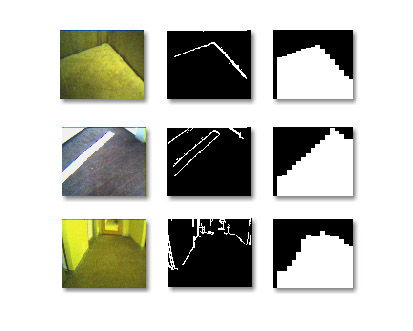
\includegraphics[scale=1]{imagens/polly_sample.jpg}
    \caption{Histograma e Detecção de Bordas de algumas imagens exemplo}
    \label{vis_fig01}
\end{figure}

\section{Correção de desvios}

De forma a corrigir eventuais desvios na movimentação do robô, causados por uma diferença de rotação entre as duas rodas, o sistema também deve identificar, na imagem, através da detecção de bordas e do mapa de cores, alguns objetos ou bordas de destaque, e caso saiam muito do lugar esperado para eles, corrigir sua rota.


% ========= %
% NAVEGAÇÃO %
% ========= %

\chapter{Navegação}

Para o robô encontrar o objeto anteriormente especificado ele deve saber se locomover dentro de um ambiente desconhecido. Para navegar no ambiente, o robô deve criar uma espécie de mapa que contenha informações que possibilitem sua locomoção no ambiente. Duas abordagens distintas são a representação de maneira global ou de maneira local \cite{conradt}.

De acordo com Jörg \cite{conradt}, a representação global procura descrever o ambiente da maneira mais fiel à realidade possível, indicando o mapa a partir de seus nodos e suas conexões, retendo o máximo de informação possível para conseguir manter uma consistência espacial global conforme o mapa vai sendo construído. A grande desvantagem da representação global é a necessidade de se reter e processar toda essa informação para criar-se o mapa, portanto conforme a quantidade de nodos aumenta, o mapa em si aumenta e a complexidade computacional também aumenta consideravelmente.

Na representação local os nodos (pontos de referência, denominados \textit{Place Agents}) possuem informações apenas do próprio local, de quais são os nodos vizinhos, possíveis pontos de interesse (objetos de destaque para identificação do nodo, por exemplo) e informações pertinentes sobre como alcançar o próximo nodo (direção, existência de obstáculos, etc.) seja este nodo já presente no mapa ou não.

Para o projeto atual, a equipe optou por utilizar a representação local, pois a abordagem global se torna ineficiente devido a sua complexidade computacional envolvida para manter a consistência do mapa. A abordagem local permite o escalonamento do sistema para permitir a ele operar em ambientes maiores.

\section{Construção do mapa}

Para a criação do mapa é utilizada principalmente a câmera \textit{CMUcam3} acoplada ao robô. A câmera é a principal responsável por adquirir informações do ambiente para a criação do mapa. Junto com a câmera, a bússola é utilizada para fornecer as direções entre um nodo e outro. Com as informações obtidas da câmera e da bússola, o robô é capaz de construir um mapa do ambiente e deve ser capaz de locomover-se dentro do ambiente, procurando o objeto desejado e desviando de obstáculos caso necessário.

Inicialmente, ao ser inicializado num novo ambiente, o robô deve criar um nodo A que será demarcado como o primeiro nodo existente no mapa. A primeira informação a ser obtida será procurar características do ambiente ou objetos próximos ao nodo para caracterizar o nodo em questão. Após obter informações do ambiente atual, o robô deve observar seus arredores e definir outros nodos alcançáveis a partir do nodo atual. O robô então deve guardar informações pertinentes sobre como chegar a cada um dos nodos vizinhos, como direção e a existência de objetos de destaque. Tais informações sobre o caminho serão guardadas em ambos os nodos envolvidos (nodo A e nodo B, inicio e destino, respectivamente). Dentre todos os nodos vizinhos, o sistema escolhe um e se locomove até ele. O processo então é repetido diversas vezes até que o mapa seja completamente montado (não existe nenhum nodo alcançável não visitado) ou o objeto seja encontrado.

\section{Roteamento}

Na representação local os nodos (pontos de referência, ou \textit{Place Agents}) possuem informações apenas do próprio local, de quais são os nodos vizinhos, possíveis pontos de interesse (objetos de destaque para identificação do nodo, por exemplo) e informações pertinentes sobre como alcançar o próximo nodo (direção, existência de obstáculos, etc.) seja este já presente no mapa ou não. Na representação local, para se alcançar um nodo já mapeado e que não seja vizinho ao atual será necessário um algoritmo de roteamento no sistema, onde cada \textit{Place Agent} pergunta por essa informação aos seus vizinhos e assim sucessivamente até que o nodo requisitado seja encontrado.

Quando o nodo requisitado é encontrado o robô traça um caminho para chegar ao local desejado, passando por nodos já existentes. 


% ========= %
% CONCLUSÃO %
% ========= %

\chapter{Conclusão}

No atual momento do projeto, a comunicação entre \textit{CMUcam3} e \textit{Arduíno} ainda não foi implementada, por esse motivo ainda não foi possível fazer os testes de exploração e identificação do objeto.

Analisando a estrutura do robô desde a parte mecânica, eletrônica e as estratégias para exploração e localização do objeto encontrado, espera-se que o robô consiga encontrar um objeto especifico e de destaque dentro de um ambiente pequeno, com as dimensões 168,2 cm por 118,9 cm.

Espera-se também conseguir implementar corretamente um código de exploração inteligente baseado em representações locais para locomoção do robô dentro do espaço determinado. Além disso, conseguir aplicar um código para reconhecer o objeto a ser encontrado utilizando características de destaque (cores fortes, forma, etc.) do objeto. Tais características do robô (locomoção e identificação) serão controladas pela câmera acoplada ao robô, a \textit{CMUcam3}.

Como continuação deste projeto, seria interessante ver o robô se locomovendo em espaços maiores e mais dinâmicos e também que o robô possa identificar objetos mais familiares ao dia a dia como algum equipamento ou molho de chaves.


%---------- Referencias ----------
\bibliography{monografia} % geracao automatica das referencias a partir do arquivo reflatex.bib

%---------- Apendices (opcionais) ----------
\apendice

\chapter{Caderno de Bordo}

\textbf{10 de Agosto}

Primeira aula da disciplina. 

\textbf{17 de Agosto}

Marcelo Teider e Matheus Araujo decidem formar a equipe, têm em mente o projeto de um robô explorador. A equipe ainda não tem os três integrantes, como sugerido para a Disciplina. Então iniciam-se negociações com outras equipes para a definição dos integrantes.

\textbf{12 de Agosto}


Após algumas conversas, as equipes da disciplina são definidas. Luis Camargo é integrado à equipe. 

\textbf{13 de Agosto}

Após a definição da equipe, a professora Myriam Delgado é convidada para nos orientar, aceitando a proposta. 

\textbf{13 de Agosto}

O projeto é então definido como a construção de um robô explorador. A intenção é “mostrar” ao robô um objeto para reconhecimento, então esse mesmo objeto é escondido de seu campo de visão e o robô deve então explorar o ambiente procurando-o. Ele deve também evitar obstáculos durante o percurso.

\textbf{24 de Agosto}

Apresentação da pré-proposta. A equipe apresentou aos professores da disciplina a pré-proposta de projeto, sendo aceita pelos professores. Como sugerido pelo professor Hugo durante a apresentação, decidimos comprar uma \textit{SmartCam}. A primeira ideia seria utilizar a \textit{CMUcam}, mas optamos por pesquisar outros modelos. 

\textbf{29/30 de Agosto}

Iniciamos as pesquisas das câmeras. Pesquisamos os modelos \textit{AVRcam}, que não está sendo produzido no momento; e alguns modelos comerciais, que foram descartados devido ao elevado custo, acima de US\$ 2000,00. Dentre os modelos \textit{CMUcam}, ficamos em dúvida entre dois modelos, \textit{CMUcam1 }e \textit{CMUcam2}. 

Fizemos um levantamento do material que será necessário para a construção do robô, como motor, chassi, bateria e microprocessador. 

\textbf{31 de Agosto}

Em conversa com o professor Hugo, optamos pela \textit{CMUcam1}; uma vez que ela atende os requisitos do projeto e tem menor custo. Os procedimentos para adquirá-la foram tomados.

Conseguimos com a equipe que desenvolveu o Robô Explorador de Labirintos 2D nessa mesma disciplina, em 2011-01, o robô emprestado. Segundo a Equipe, uma das Pontes H do robô apresenta problemas, precisaremos solucioná-lo. 

Precisamos agora decidir e conseguir o microcontrolador para o Robô. Os da plataforma \textit{Arduíno} apresentam possibilidade de comunicação com a câmera via software e pela familiaridade dos membros da equipe podem se tornar uma boa escolha.

\textbf{5 de Setembro}

Pegamos o robô com a equipe do semestre passado. Sem problemas com a ponte H, o robô não apresenta nenhum problema mecânico ou elétrico-eletrônico. Estamos utilizando o mesmo microcontrolador da equipe, um \textit{ATMEGA 328P} em  uma placa \textit{Arduíno Duemilanove}. 

\textbf{ 7 de Setembro}

Desenvolvemos uma API para controle do hardware do Robô. Fizemos uma classe \textit{Robot} em C++ com funções pré-definidas como \textit{startrobot}, \textit{forward}, \textit{turnleft}. No código a ser desenvolvido não necessitaremos controlar o robô diretamente, apenas através dessa classe.

\textbf{12 de Setembro}

Por indicação de nossa orientadora, conhecemos o trabalho \textit{A Distributed Cognitive Map for Spatial Navigation Based on Graphically Organized Place Agents}, de Jörg Conradt e Rodney Douglas, e por orientação do professor Luiz Merkle com um algoritmo de busca recursiva em um espaço bidimensional pelas quatro direções cardeais através de pilha, no livro \textit{Data Structures - An advanced approach using C}.

\textbf{21 de Setembro}

Definida a data da banca final, 7 de Dezembro. 

Por orientação do professor Hugo, entramos em contato com diversos artigos de Prestes, Lowe, Bay e Artolazabal.

\textbf{23 a 28 de Setembro}

Escrita do relatório de Qualificação, entregue aos professores no dia 28. Percebemos a necessidade de usar uma bússola como sensor para definir a direção em que se encontra o robô.

\textbf{28 de Setembro}

Entrega da Qualificação aos professores da Disciplina. Conseguimos emprestado com o professor Hugo duas bússolas \textit{Dinsmore}, uma digital e outra analógica. Durante a próxima semana faremos os testes para definir qual iremos usar. A bússola será integrada ao sistema através da placa do \textit{Arduíno}.

\textbf{30 de Setembro}

Foram encontrados problemas com o interfaceamento entre a bússola e o arduíno devido a diferentes níveis de tensão e corrente, será necessário construir um conversor DC-DC para fazer a integração.

\textbf{6 de Outubro}

Após orientação do professor Hugo e pesquisa de outros projetos, fizemos o primeiro experimento com a bússola e obtivemos 5 [V] na saída, o que possibilita interfaceamento direto com o arduíno. 

\textbf{12 de Outubro}

Construímos um \textit{shield} para a bússola, possibilitando conectá-la ao Arduíno.

\textbf{14 de Outubro}

A câmera foi finalmente enviada de Hong Kong. A previsão de entrega é de um mês, precisamos elaborar um plano B caso a câmera não chegue a tempo da finalização do projeto.

\textbf{15 de Outubro}

Conectamos o \textit{shield} da bússola ao Arduíno; tivemos alguns problemas de mau contato com os cabos, mas o robô é capaz de interpretar as informações fornecidas pela bússola e segue os comandos que lhe foram dados. 

\textbf{18 de Outubro}

Tivemos uma reunião com nossa orientadora, Prof. Myriam, onde apresentamos o estado atual do projeto e elaboramos um segundo plano, caso a câmera não chegue. Iremos utilizar os sensores do projeto passado, cinco pares de leds emissor/receptor, e construir uma pasta com marcas de diferentes cores perceptíveis pelo robô, onde ele deverá construir um mapa cognitivo. 

\textbf{19 de Outubro}

A câmera chegou! Iremos começar os testes com ela em breve. Precisaremos de um cabo serial ou um adaptador para comunicação com a placa e também de baterias para alimentação da mesa, 6V.

\textbf{26 de Outubro}

Compramos um adaptador para o cabo de comunicação e um suporte para quatro pilhas AA que servirá como alimentação.

Conseguimos compilar e gravar os códigos de exemplo na câmera.

\textbf{2 de Novembro}

Estamos estudando a comunicação da \textit{CMUCam} com o \textit{Arduíno}.

\textbf{9 de Novembro}

Concentramos nossas atenções na finalização da primeira versão da monografia.


\chapter{Descritivo}

Esse apêndice tem como intuito descrever de maneira sucinta o que foi realizado durante o projeto, e pode ser utilizado em trabalhos futuros como referência rápida.

O objetivo inicial da equipe era construir um robô que pudesse se localizar em um ambiente controlado e conseguisse encontrar um objeto especificado; durante o projeto, a bola laranja foi definida como o objeto a ser pesquisado.

Houve algumas dificuldades na aquisição da câmera, inicialmente, a equipe optou pela \textit{CMUCam1}, por atender os requisitos do projeto e ser mais barata. No entanto, nenhum fornecedor da câmera possuia o modelo mais simples da \textit{CMUCam}, o mesmo aconteceu com a \textit{CMUCam2}, sendo necessário então adquirir a \textit{CMUCam3} junto a um fornecedor em Hong Kong.

A entrega da câmera atrasou devido a dos funcionários dos Correios no Brasil.

Enquanto a câmera não chegava, a equipe trabalhou com o robô que já havia sido construído, e implementou a biblioteca de controle do mesmo. Nesse período foram feitos os testes com a bússola também. A equipe conseguiu integrá-la ao \textit{Arduino} e chegou a fazer alguns testes de movimento do robô a partir de informações que eram obtidas através dela.

Com a câmera em mãos, foram feitos os testes dos algoritmos de reconhecimento da \textit{CMUCam3}. O programa exemplo usado para identificação foi o \textit{simple-track-color}. Este programa é capaz de, a partir de uma faixa RGB, identificar dentro da imagem onde está a cor e retorna como parâmetro dois pontos de um retângulo onde a cor está contida, o centróide da cor, i.e., o ponto onde há maior concentração daquela cor, e a densidade da cor dentro daquele retângulo.

Com um algoritmo rudimentar de identificação funcionando, a equipe se concentrou em desenvolver o sistema de comunicação \textit{Arduino-CMUCam}. Fisicamente, foi utilizada a porta serial da \textit{CMUCam}, a mesma que ela utiliza para comunicar com o computador, e os pinos 0 e 1 do \textit{Arduino}. Nos testes feitos pela equipe, aparentemente não havia uma relação direta entre o que era enviado pela câmera e o que era recebido pelo \textit{Arduino}; no entanto, havia a integridade da informação. Ou seja, o que era enviado pela câmera era sempre recebido da mesma forma pelo \textit{Arduino}, então a equipe levantou uma tabela de relação e implementou o sistema de comunicação.

Quando os dois módulos descritos anteriormente já estavam funcionando, o prazo de entrega do projeto já estava muito próximo e a equipe então reduziu o escopo do projeto e o objetivo passou a ser identificar o objeto e fazer o robô se movimentar até ele. Para isso, foi elaborado um algoritmo simples de navegação. 

Esse algoritmo movimenta o robô em direção à bola sem no entanto evitar obstáculos. O robô para quando a bola está suficientemente próxima. Os parâmetros de decisão de parada, virar para a esquerda ou direita, movimentar para a frente foram obtidos de maneira experimental. 
i
Todo o código desenvolvido pela equipe está disponível no repositório: $$ http://github.com/matheusaraujo/oficina2-robocam $$

Como projetos futuros, a equipe sugere implementar um algoritmo inteligente de navegação e aprimorar a percepção, utilizando outras informações além da cor do objeto, como detecção de bordas e histograma também. Com relação ao projeto mecânico do robô, acredita-se que foi atingido um nível satisfatório, precisando apenas alguns ajustes pequenos principalmente com relação aos diversos fios do robô que eventualmente podem atrapalhar os movimentos. Outro ponto a ser explorado é a integração das informações da bússola ao algoritmo de exploração.


%\chapter{Nome do Ap\^endice}

%Use o comando {\ttfamily \textbackslash apendice} e depois comandos {\ttfamily \textbackslash chapter\{\}}
%para gerar t\'itulos de ap\^en-dices.


% ---------- Anexos (opcionais) ----------
%\anexo
%\chapter{Nome do Anexo}

%Use o comando {\ttfamily \textbackslash anexo} e depois comandos {\ttfamily \textbackslash chapter\{\}}
%para gerar t\'itulos de anexos.


% --------- Lista de siglas --------
%\textbf{* Observa\c{c}\~oes:} a lista de siglas nao realiza a ordenacao das siglas em ordem alfabetica
% Em breve isso sera implementado, enquanto isso:
%\textbf{Sugest\~ao:} crie outro arquivo .tex para siglas e utilize o comando \sigla{sigla}{descri\c{c}\~ao}.
%Para incluir este arquivo no final do arquivo, utilize o comando \input{arquivo.tex}.
%Assim, Todas as siglas serao geradas na ultima pagina. Entao, devera excluir a ultima pagina da versao final do arquivo
% PDF do seu documento.


%-------- Citacoes ---------
% - Utilize o comando \citeonline{...} para citacoes com o seguinte formato: Autor et al. (2011).
% Este tipo de formato eh utilizado no comeco do paragrafo. P.ex.: \citeonline{autor2011}

% - Utilize o comando \cite{...} para citacoeses no meio ou final do paragrafo. P.ex.: \cite{autor2011}



%-------- Titulos com nomes cientificos (titulo, capitulos e secoes) ----------
% Regra para escrita de nomes cientificos:
% Os nomes devem ser escritos em italico, 
%a primeira letra do primeiro nome deve ser em maiusculo e o restante em minusculo (inclusive a primeira letra do segundo nome).
% VEJA os exemplos abaixo.
% 
% 1) voce nao quer que a secao fique com uppercase (caixa alta) automaticamente:
%\section[nouppercase]{\MakeUppercase{Estudo dos efeitos da radiacao ultravioleta C e TFD em celulas de} {\textit{Saccharomyces boulardii}}
%
% 2) por padrao os cases (maiusculas/minuscula) sao ajustados automaticamente, voce nao precisa usar makeuppercase e afins.
% \section{Introducao} % a introducao sera posta no texto como INTRODUCAO, automaticamente, como a norma indica.


\end{document}
